\documentclass{beamer}

\usefonttheme{serif}

\setbeamertemplate{footline}[frame number]{}
\setbeamertemplate{navigation symbols}{}

\usecolortheme{default}
\setbeamercolor{block title}{bg=lily!20,fg=black}
\setbeamercolor{block body}{bg = blue!10, fg = black}
\setbeamertemplate{itemize item}[square]
\setbeamercolor{itemize item}{fg = cyan}
\setbeamercolor{enumerate item}{fg = cyan}

\usetheme{default}

%\setbeamercolor{titlelike}{fg=cyan}
%Information to be included in the title page:
\title{Sample title}
\author{Anonymous}
\institute{Overleaf}
\date{2021}

\title[About Beamer] %optional
{Helium–Neon Laser}

%\subtitle{A short story}

\author[Arthur, Doe] % (optional, for multiple authors)
{A.~Simankovich \and D.~Dedkov }

\institute[VFU] % (optional)
{
	Moscow Institute of Physics and Technology
}

\date[VLC 2023] % (optional)
%{Very Large Conference, April 2021}

%\logo{\includegraphics[height=1cm]{overleaf-logo}}

\begin{document}
	
	\frame{\titlepage}
	
	\begin{frame}
		\frametitle{Abstract}
		TODO

	\end{frame}
	
	\begin{frame}
		\frametitle{General laser scheme}
		\begin{figure}
			\centering
			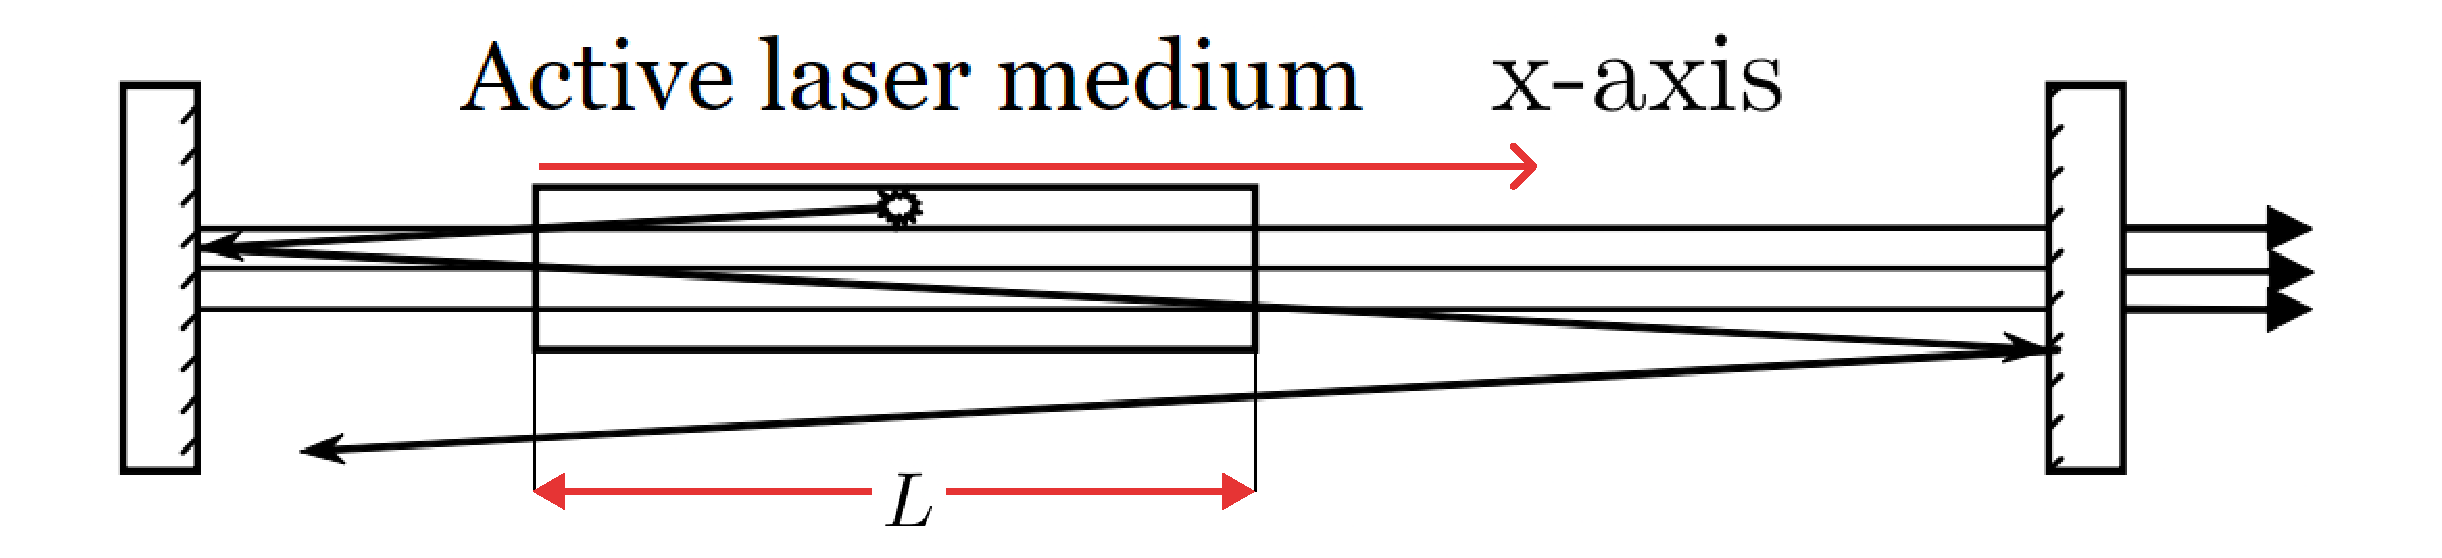
\includegraphics[width=1\linewidth]{res/general_laser_scheme.pdf}
			\caption{General laser scheme}
			\label{fig:general_laser_scheme}
		\end{figure}
		
	\end{frame}
	
	\begin{frame}
		\frametitle{Einstein coefficients}
		\begin{figure}
			\centering
			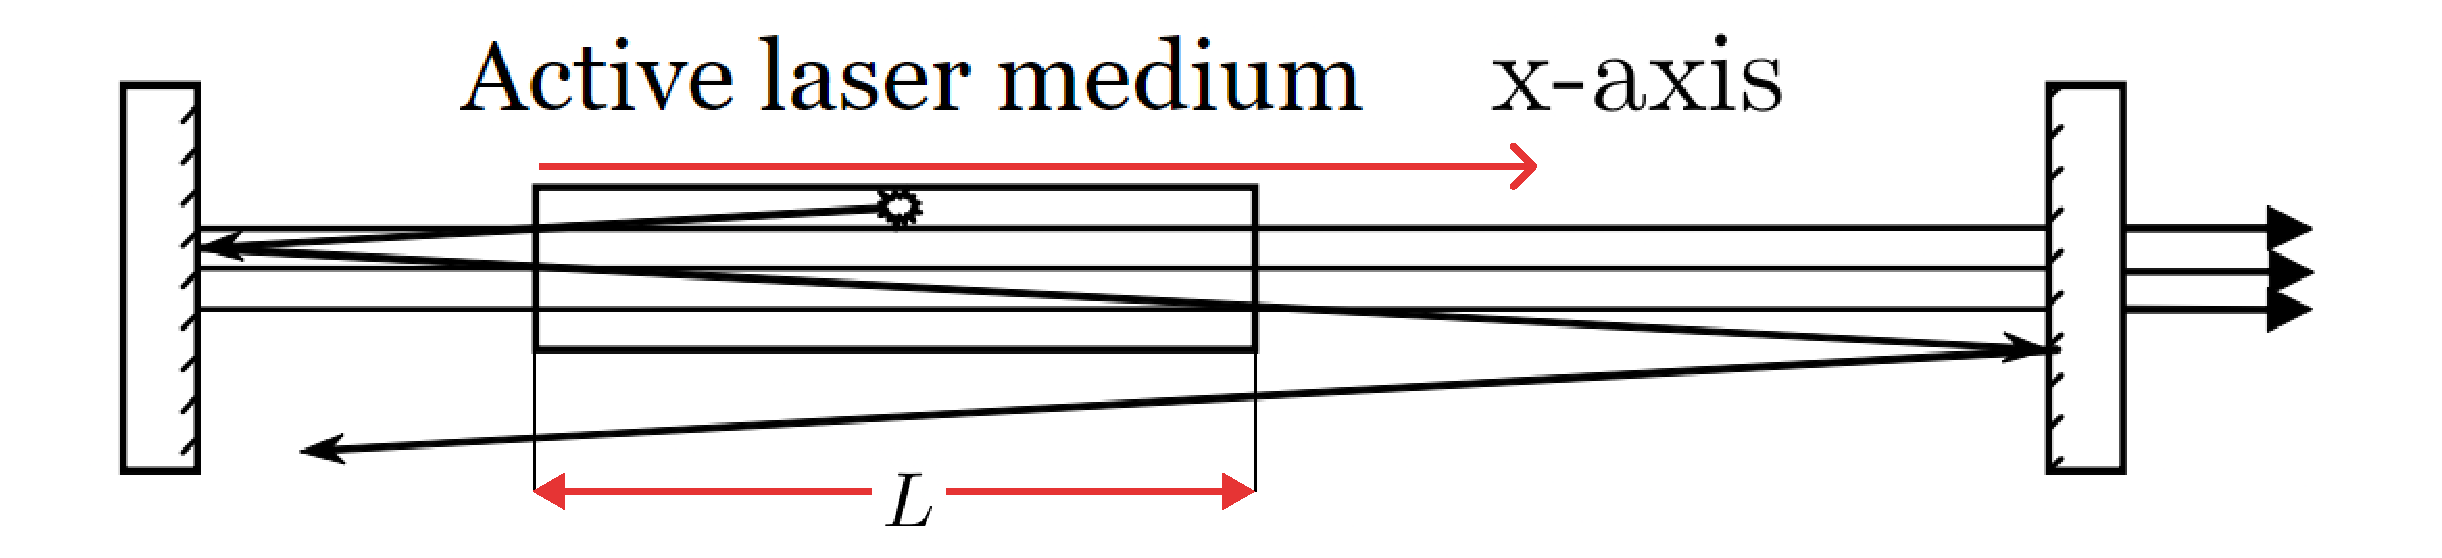
\includegraphics[width=1\linewidth]{res/general_laser_scheme.pdf}
			\caption{General laser scheme}
			\label{fig:general_laser_scheme}
		\end{figure}
		
	\end{frame}
	
	\begin{frame}
		\frametitle{Elementary processes}
		\begin{figure}
			\centering
			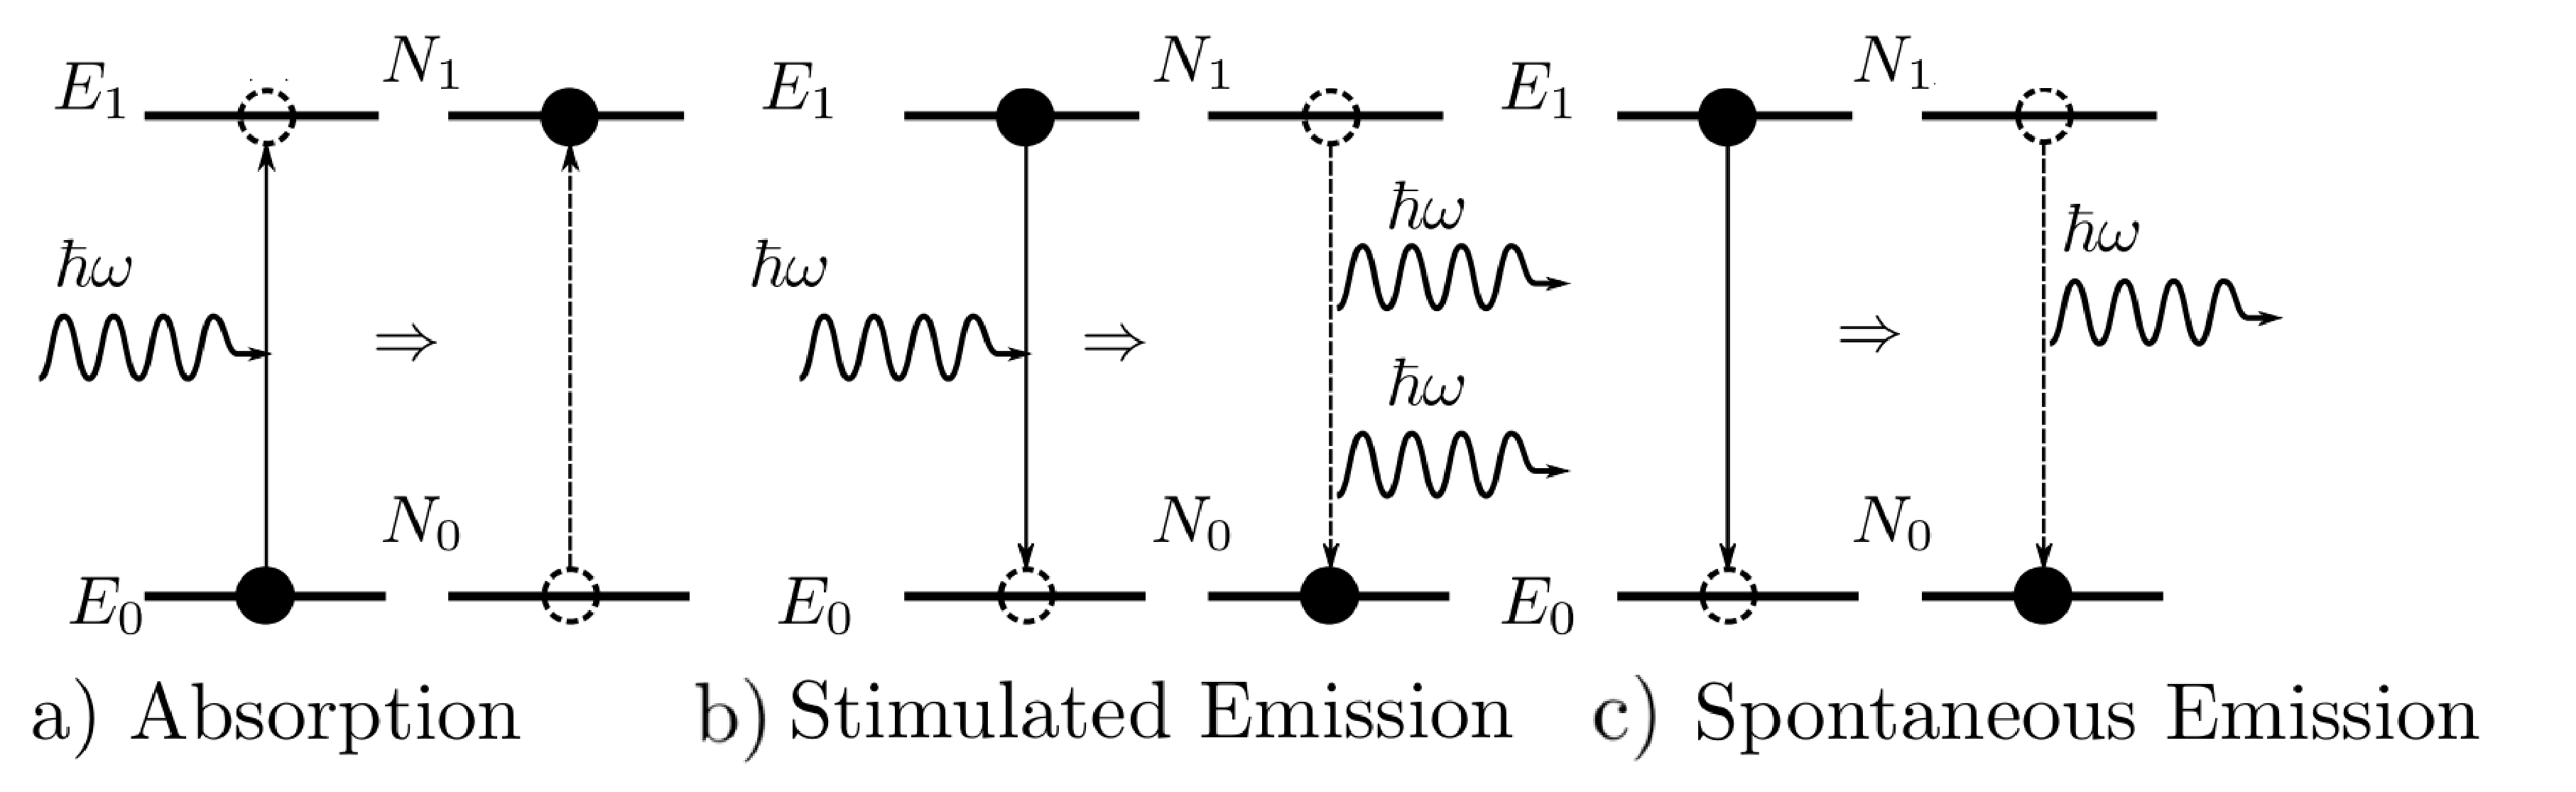
\includegraphics[width=1\linewidth]{res/emission_types.pdf}
		\end{figure}
	
		\begin{table}
			\centering
			\footnotesize
			\begin{tabular}{p{0.33\linewidth}p{0.32\linewidth}p{0.32\linewidth}}

				$\left(\frac{dN_0}{dt}\right)_{\text{abs}} = - B_{01} N_0 \rho(\omega)$  &
				$\left(\frac{dN_0}{dt}\right)_{\text{stim}} = B_{10} N_1 \rho(\omega)$   &  
				$\left(\frac{dN_0}{dt}\right)_{\text{spon}} = - A_{10} N_1$ \\ & & \\
				 Einstein coefficients are the same $B_{01} = B_{10} = B$ & 
				 phase, direction and frequency of emitted and external photons are identical. &
				 photons radiate independently in all directions. $\frac{dN_0}{dt}$ \textbf{does not} depend on $\rho(\omega)$. \\
			\end{tabular}
		\end{table}
		
		\footnotesize
		Where $\rho(\omega)$ -- spectral energy density of the isotropic radiation field at the frequency of the transition.
	\end{frame}

	\begin{frame}
	\frametitle{Gain}
	
	\begin{figure}
		\centering
		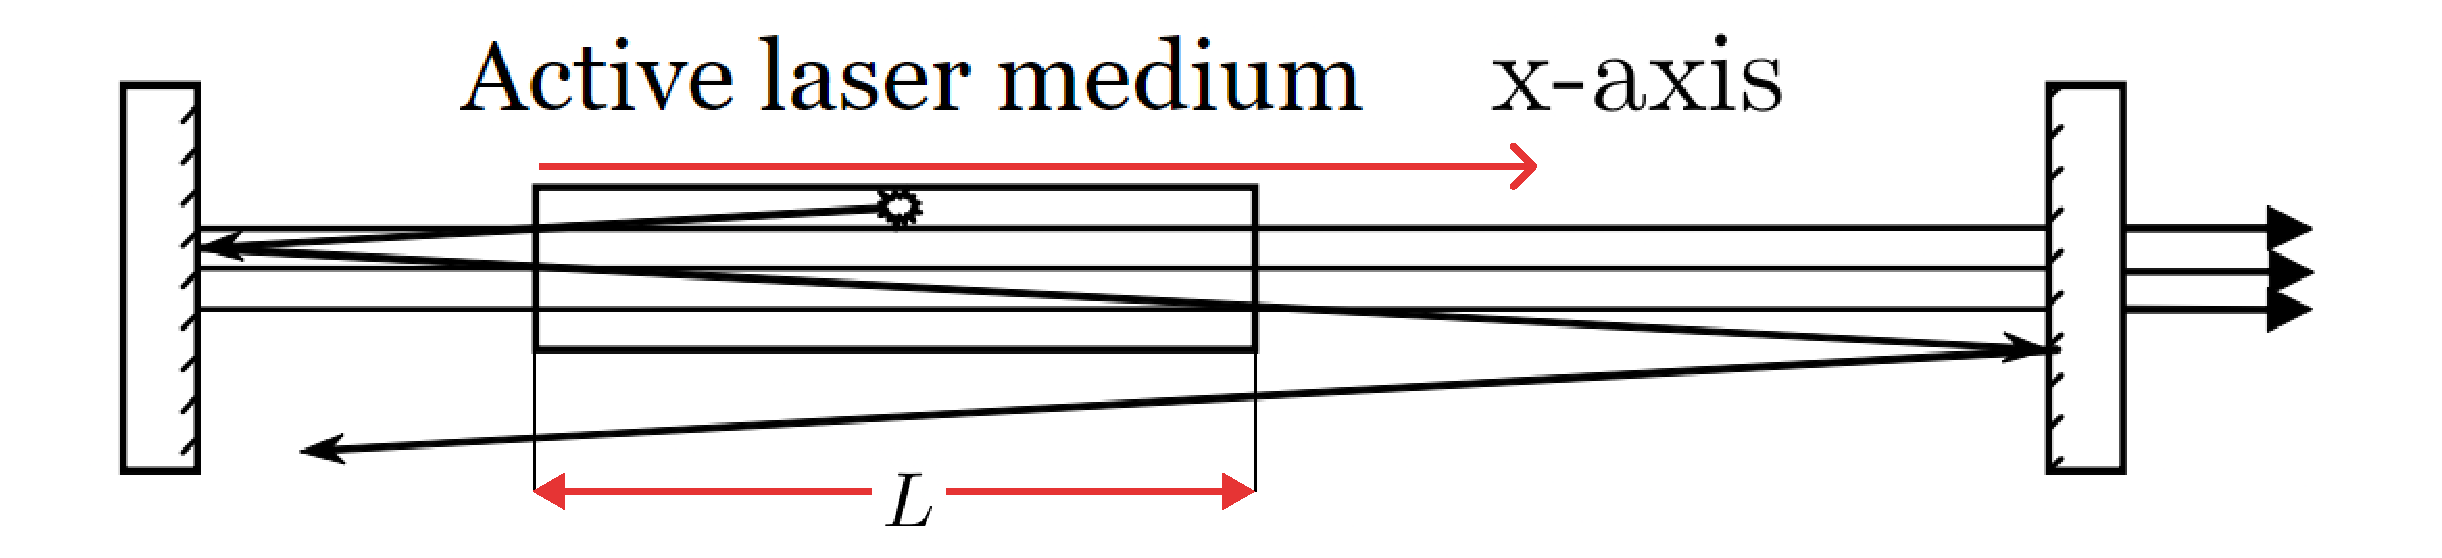
\includegraphics[width=1\linewidth]{res/general_laser_scheme.pdf}
		\caption{General laser scheme}
		\label{fig:general_laser_scheme}
	\end{figure}
	Beer–Lambert–Bouguer law states that intensity of light $I(x)$ changes:
	$$I(x) = I_0 \exp({\gamma x}),$$
	
	where $\gamma$ -- medium gain coefficient. With length $L$ gain per period is called \textbf{laser gain}:
	
	$$G = \exp{(2\gamma L)}.$$
	\end{frame}
	
	\begin{frame}
		\frametitle{Population inversion}
		The fact that the number of spontaneously emitted photons does not depend on  $\rho(\omega)$ gives us a reason to neglect $\left(\frac{dN_0}{dt}\right)_{\text{spon}}$ term. Number of photons emitted at a time $dt$:
		
		\begin{equation} \label{eq1}
			\begin{split}
				\frac{dN}{dt} & = \left(\frac{dN_0}{dt}\right)_{\text{abs}} + \left(\frac{dN_0}{dt}\right)_{\text{stim}} =  B (N_1 - N_0) \rho(\omega)
			\end{split}
		\end{equation}

		Therefore:
		\begin{equation}
			\gamma = \frac{dI}{I} = \frac{dN \cdot \hbar\omega}{\rho(\omega)} = B\frac{\hbar\omega }{v} (N_1 - N_0), 
		\end{equation}
		where $v = \frac{c}{n}$ -- speed of light inside medium.
		
		\vspace*{20px}
		\centering
		$\gamma$ is positive if $N_1 > N_0$. This laser principle is called \textbf{population inversion}
	\end{frame}


\begin{frame}
	\frametitle{Experimental setup}
	\begin{figure}
		\centering
		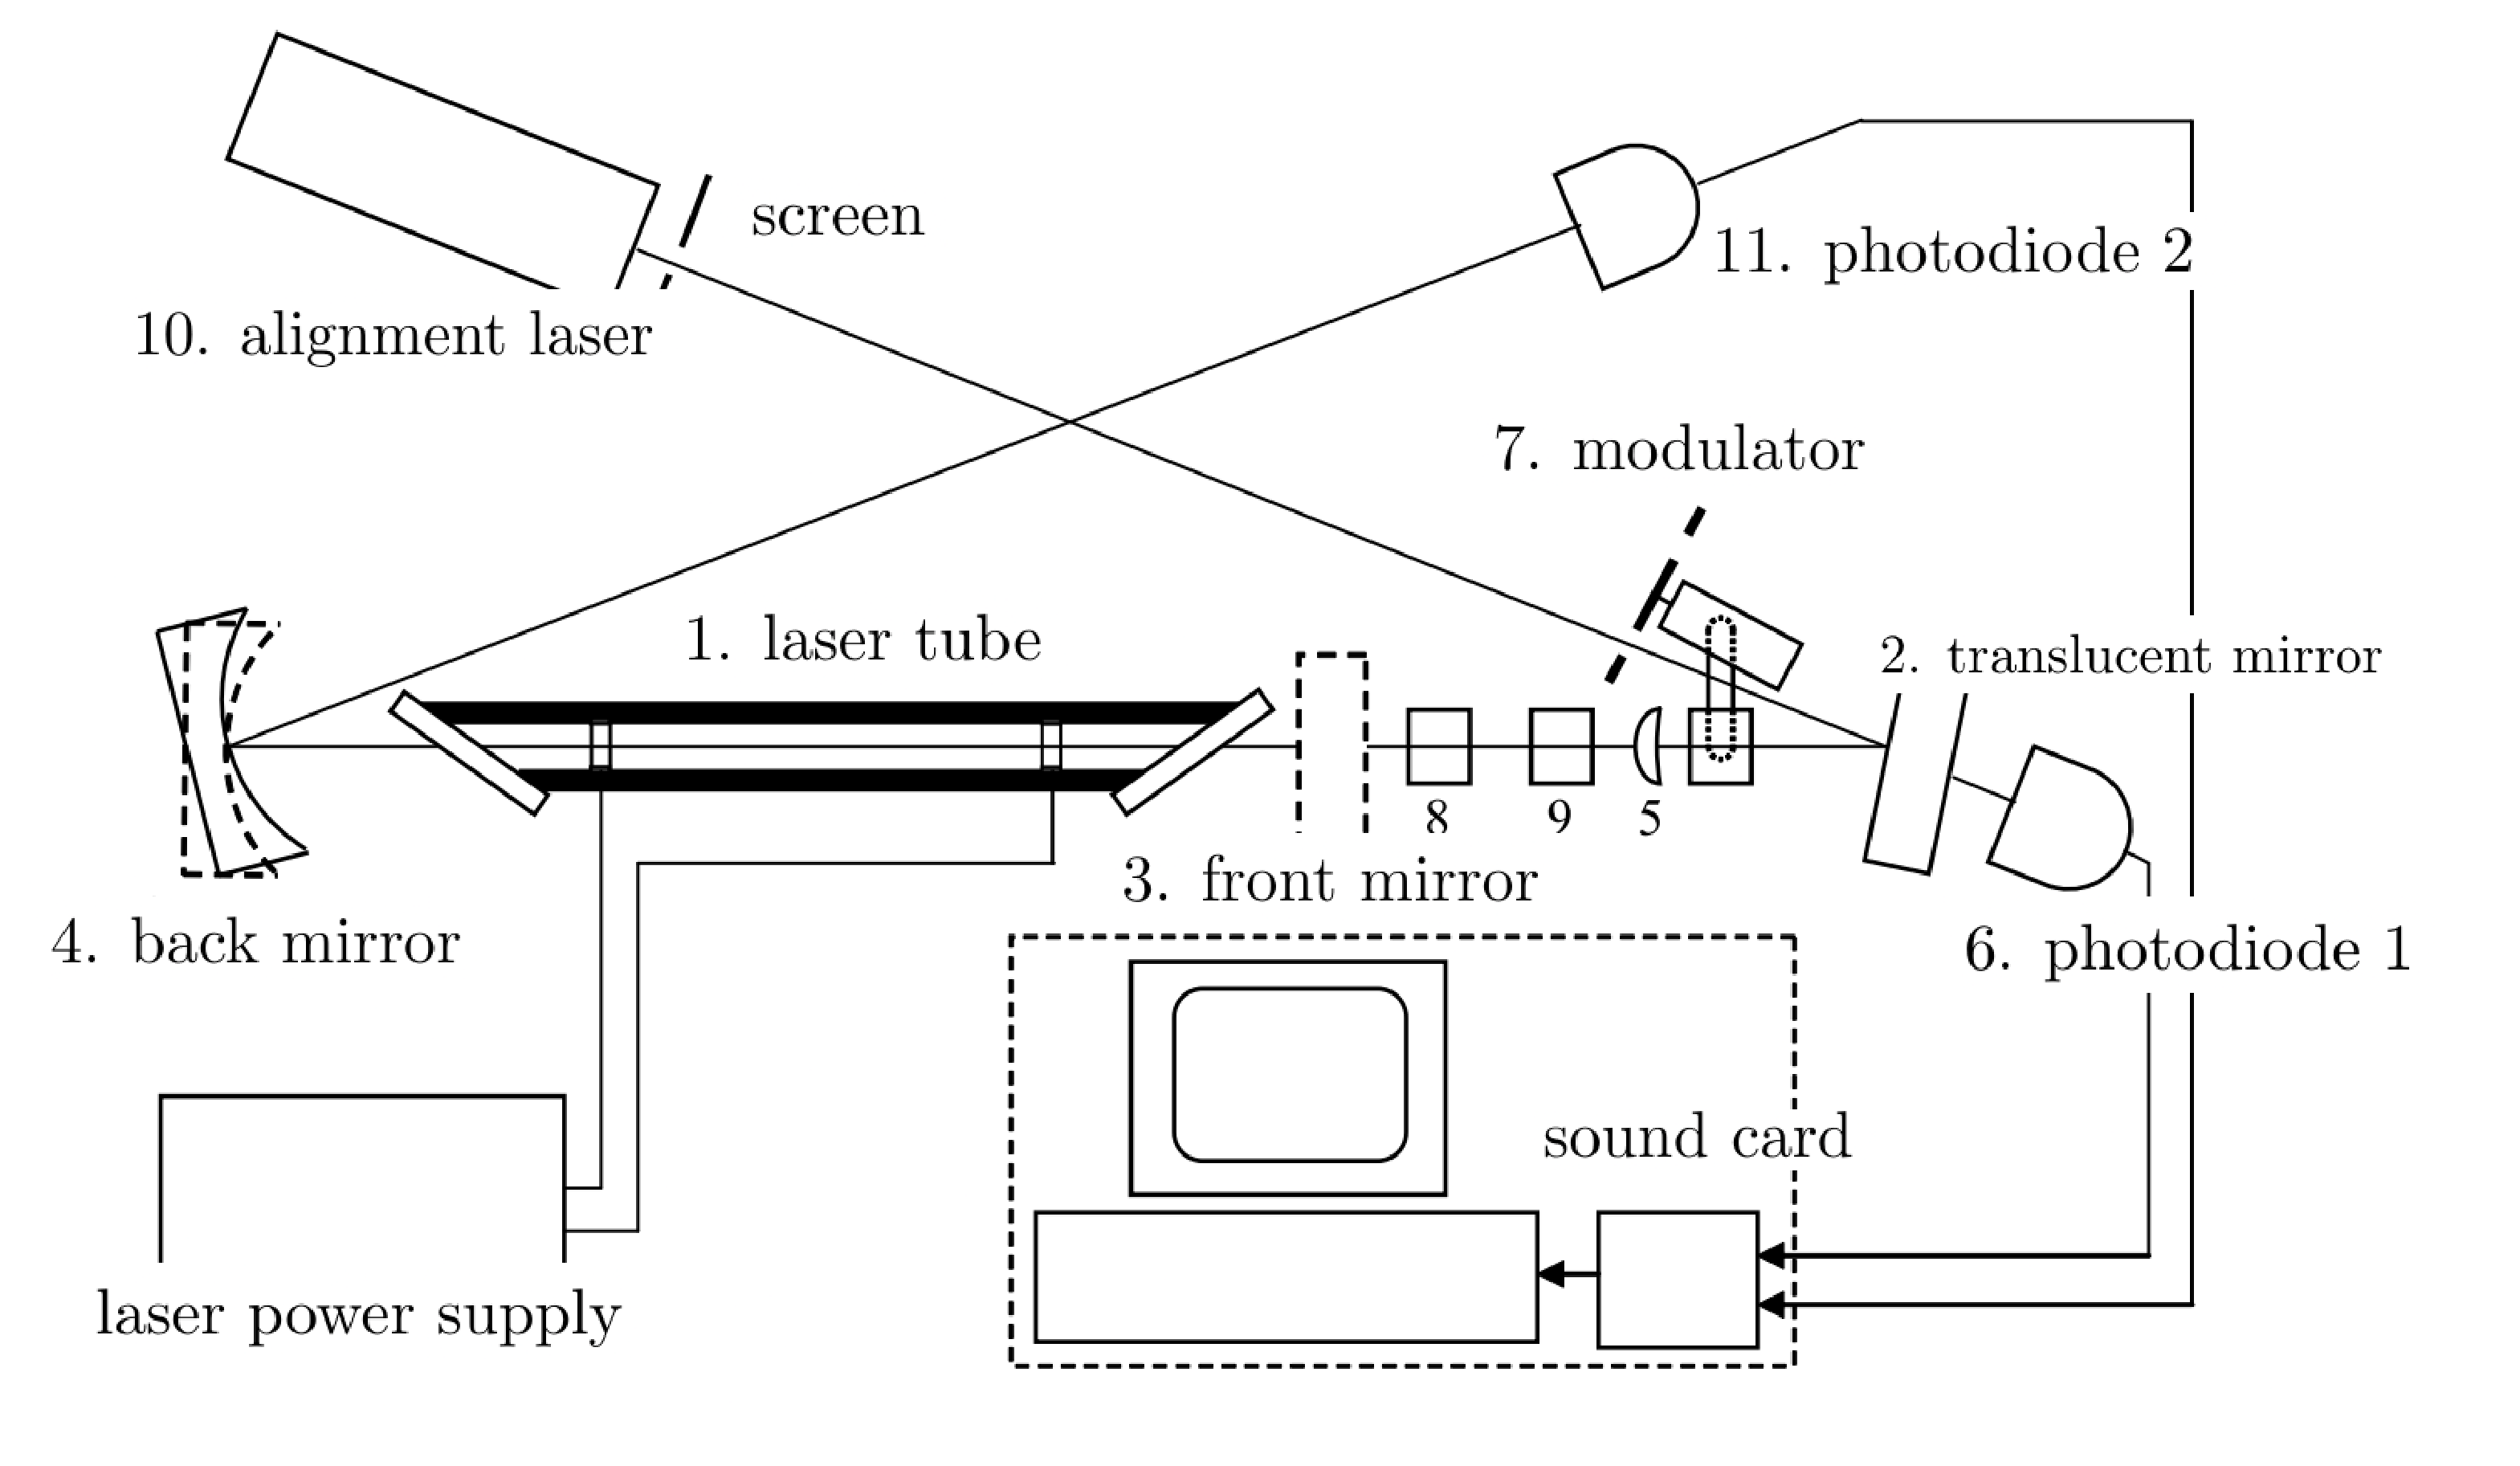
\includegraphics[width=1.1\linewidth]{res/experimental_setup.pdf}
	\end{figure}

\end{frame}

\begin{frame}
	\frametitle{Polarization of Laser Emission}
	\begin{figure}
		\centering
		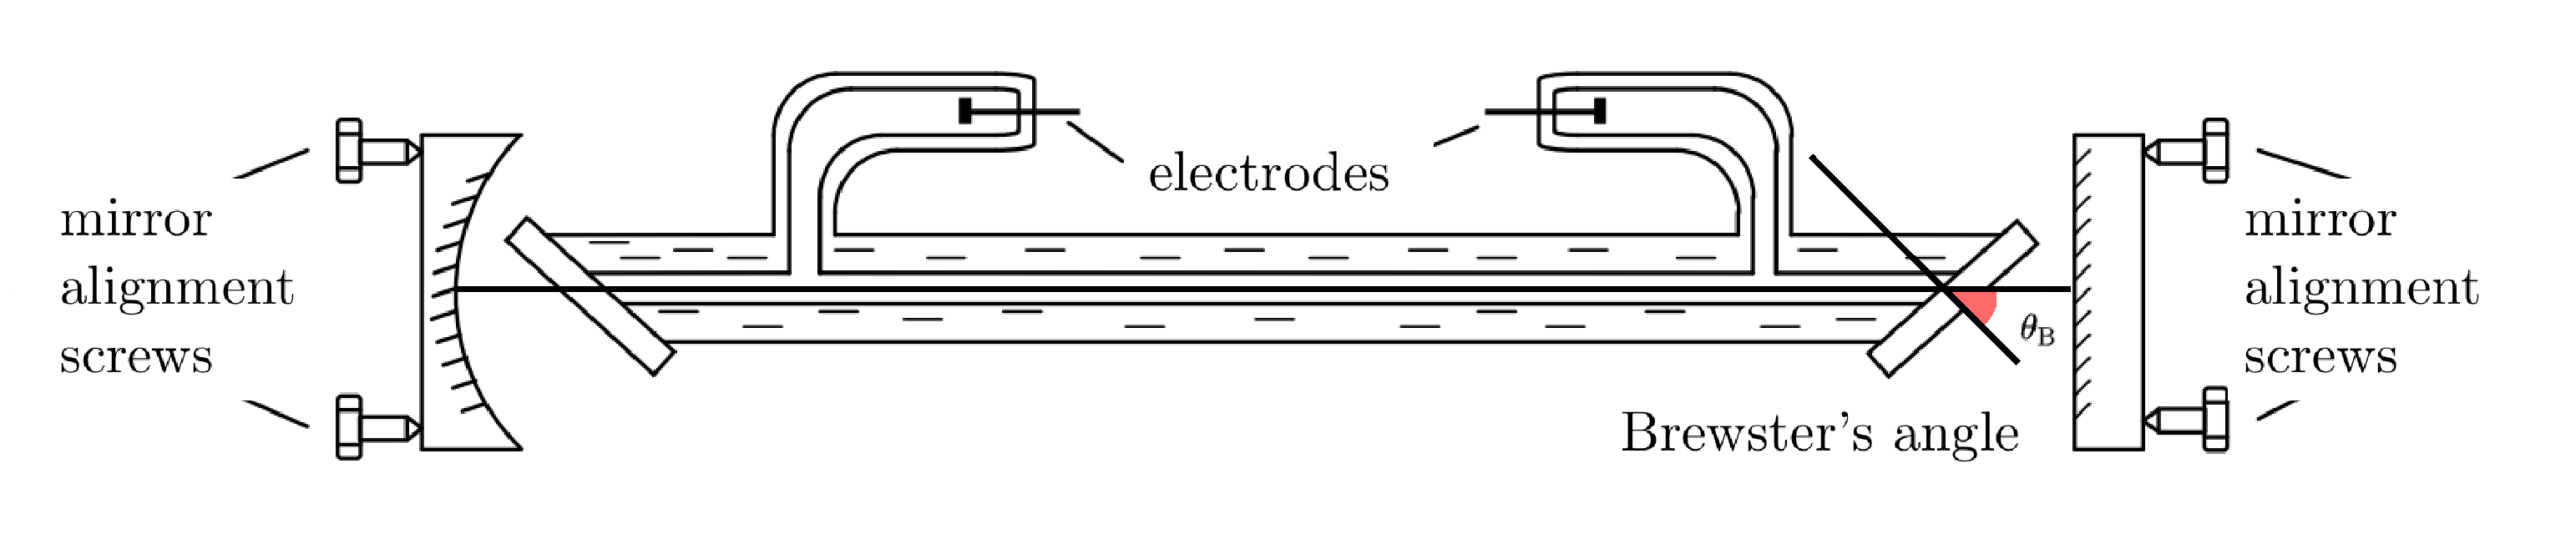
\includegraphics[width=1\linewidth]{res/brewster_setup.pdf}
	\end{figure}
	
	\begin{columns}
		\begin{column}{0.3\textwidth}
			\begin{figure}
				\centering
				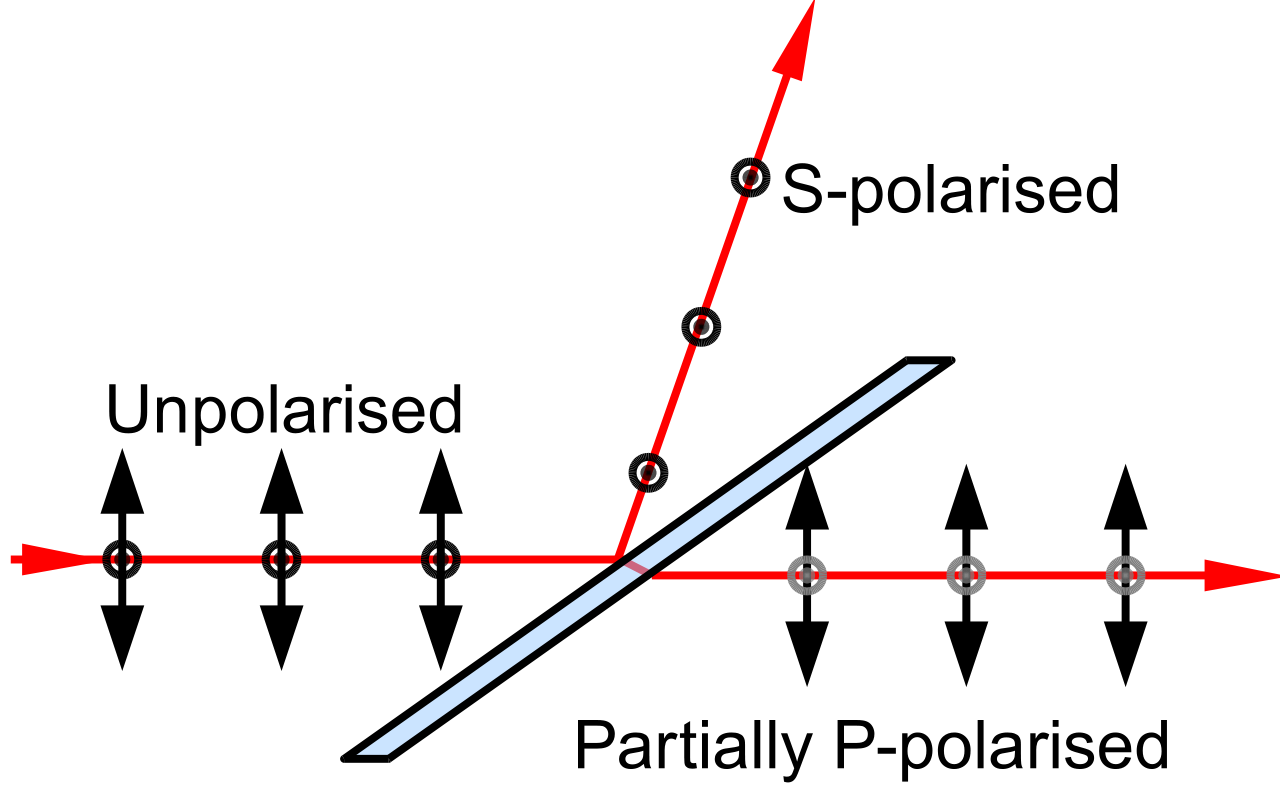
\includegraphics[width=1\linewidth]{res/brewsters-angle.svg}
			\end{figure}
		\end{column}
		\begin{column}{0.7\textwidth}
			To remove reflections from laser's windows the Brewster's angle property can be used:
			$$r_p = \frac{E_r}{E_i} = \frac{n_2 \cos{\theta_i} - n_1 \cos{\theta_t}}{n_2 \cos{\theta_i} + n_1 \cos{\theta_t}}\bigg\rvert_{\theta_i = \theta_B} = 0$$
		\end{column}
	\end{columns}	
	

	
\end{frame}


	\begin{frame}
	\frametitle{Gain}
	The fact that the number of spontaneously emitted photons does not depend on  $\rho(\omega)$ gives us a reason to neglect $\left(\frac{dN_0}{dt}\right)_{\text{spon}}$ term. Number of 
	
	1. laser tube
	
	laser power supply
	
	4. back mirror
	
	3. front mirror
	
	sound card
	
	2. translucent mirror
	
	6. photodiode 1
	
	11. photodiode 2
	
	7. modulator
	
	screen
	
	10. alignment laser
	Brewster's angle


\end{frame}
\begin{frame}
	\begin{columns}
		\begin{column}{0.2\textwidth}
			mirror alignment screws
			
			
		\end{column}
		\begin{column}{0.4\textwidth}
		mirror alignment screws
		\end{column}
	\end{columns}
\end{frame}
	
\end{document}